\begin{activity} \label{A:11.8.5} Set up an iterated integral in cylindrical coordinates to find the volume of the solid bounded below by the cone $z = \sqrt{x^2+y^2}$ and above by the cone $z = 4 - \sqrt{x^2+y^2}$. A picture is shown in Figure \ref{F:11.8.Cylindrical_ex2}.
\begin{figure}[ht]
\begin{center}
%\resizebox{!}{2.75in}{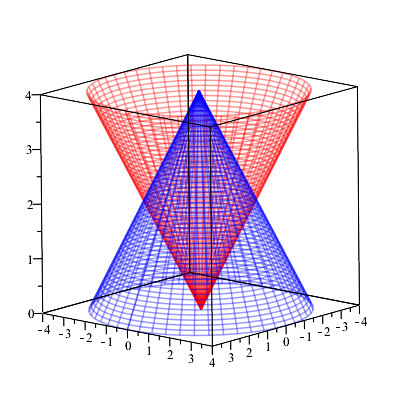
\includegraphics{11_8_Cylindrical_ex2}}
  
\includegraphics{figures/fig_11_8_two_cones.eps}
\end{center}
\caption{A solid bounded by the cones $z = \sqrt{x^2+y^2}$  and $z = 4 - \sqrt{x^2+y^2}$.}
\label{F:11.8.Cylindrical_ex2}
\end{figure}

\end{activity}
\begin{smallhint}

\end{smallhint}
\begin{bighint}

\end{bighint}
\begin{activitySolution}
In cylindrical coordinates the cones are $z=r$ and $z=4-r$. So we have $r \leq z \leq 4-r$. Now $z=r$ and $z=4-r$ intersect when $r = 4-r$ or when $r=2$. So the projection of this solid in the $xy$-plane is the disk $0 \leq r \leq 2$ and $0 \leq \theta \leq 2\pi$. So an iterated integral in cylindrical coordinates that gives the volume of this solid is
\[\int_0^{2\pi} \int_0^2 \int_{r}^{4-r} r \, dz \, dr \, d\theta.\]
\end{activitySolution}
\aftera
